\documentclass[12pt, oneside, a4paper]{article}
\usepackage[a4paper, left = 2cm, right = 2cm, top=3cm, bottom=2.5cm]{geometry}
\usepackage{fancyhdr}
\usepackage{graphicx}
\usepackage{mathtools}
\usepackage{amsfonts}
\usepackage{amsthm}
\usepackage{amsmath}
\usepackage{enumitem}
\usepackage{pgfplots}
\pgfplotsset{compat=newest}
\usepackage{bm}
\usepackage{gensymb}
\usepackage{pgfplotstable}
\usepackage{float}
\usepackage{tikz}
\makeatletter
\renewcommand*\env@matrix[1][*\c@MaxMatrixCols c]{%
	\hskip -\arraycolsep
	\let\@ifnextchar\new@ifnextchar
	\array{#1}}
\makeatother
\usepackage{amssymb}
\newcommand{\divides}{\mid}

%\renewcommand{\familydefault}{\sfdefault}
\renewcommand{\rmdefault}{ptm}


\pagestyle{fancy}
\fancyhf{}
\renewcommand{\headrulewidth}{0pt}
\fancyhead[C]{\thepage\\}
\fancyhead[R]{ID: 107664618 \\ Joy \underline{HU} \\ UPI: mhu138}

\begin{document} 
	\begin{enumerate}
		\item \begin{enumerate}[label = (\alph*)]
			
			\item Let $X$ be the number of Ardent-voters out of $1000$ respondents.
			\begin{align*}
			X &\sim \text{Binomial}(1000,p_A) \\
			H_0 &: p_A = 0.4 \\
			H_1 & : p_A \neq 0.4 & \text{(two-sided test)}
			\end{align*}

			\item  Under $H_0$, we have $X \sim \text{Binomial}(1000,0.4)$, The probability function of $X$ peaks at about $1000 \times 0.4 = 400$
\begin{figure}[H]
	\centering
	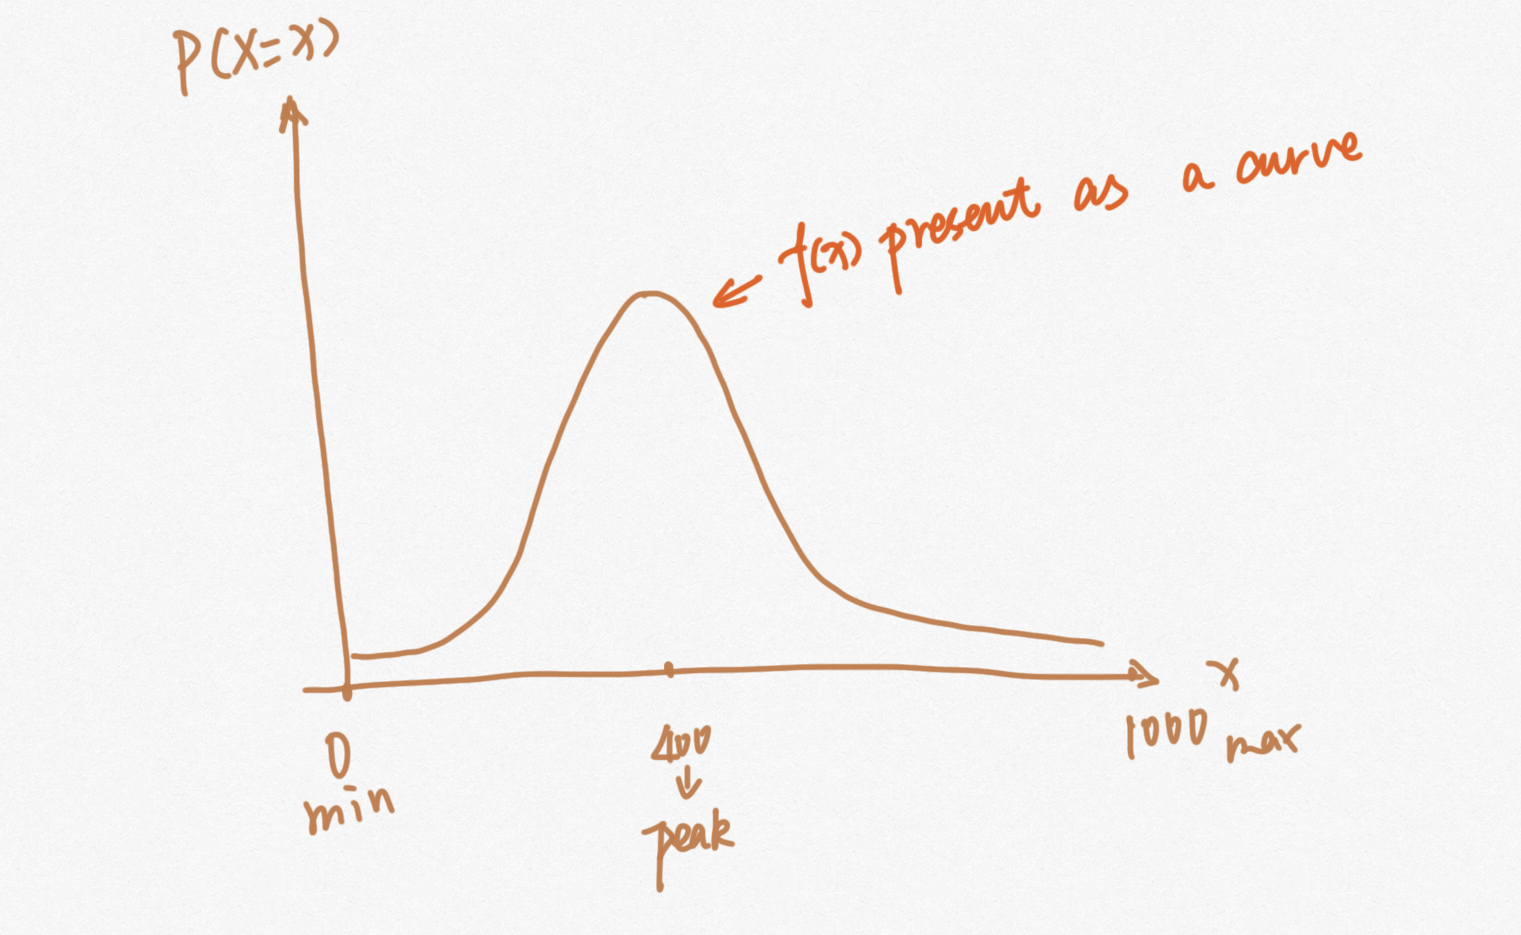
\includegraphics[width=0.8\linewidth]{1b}
	\label{fig:1b}
\end{figure}
			
			\item \begin{figure}[h]
				\centering
				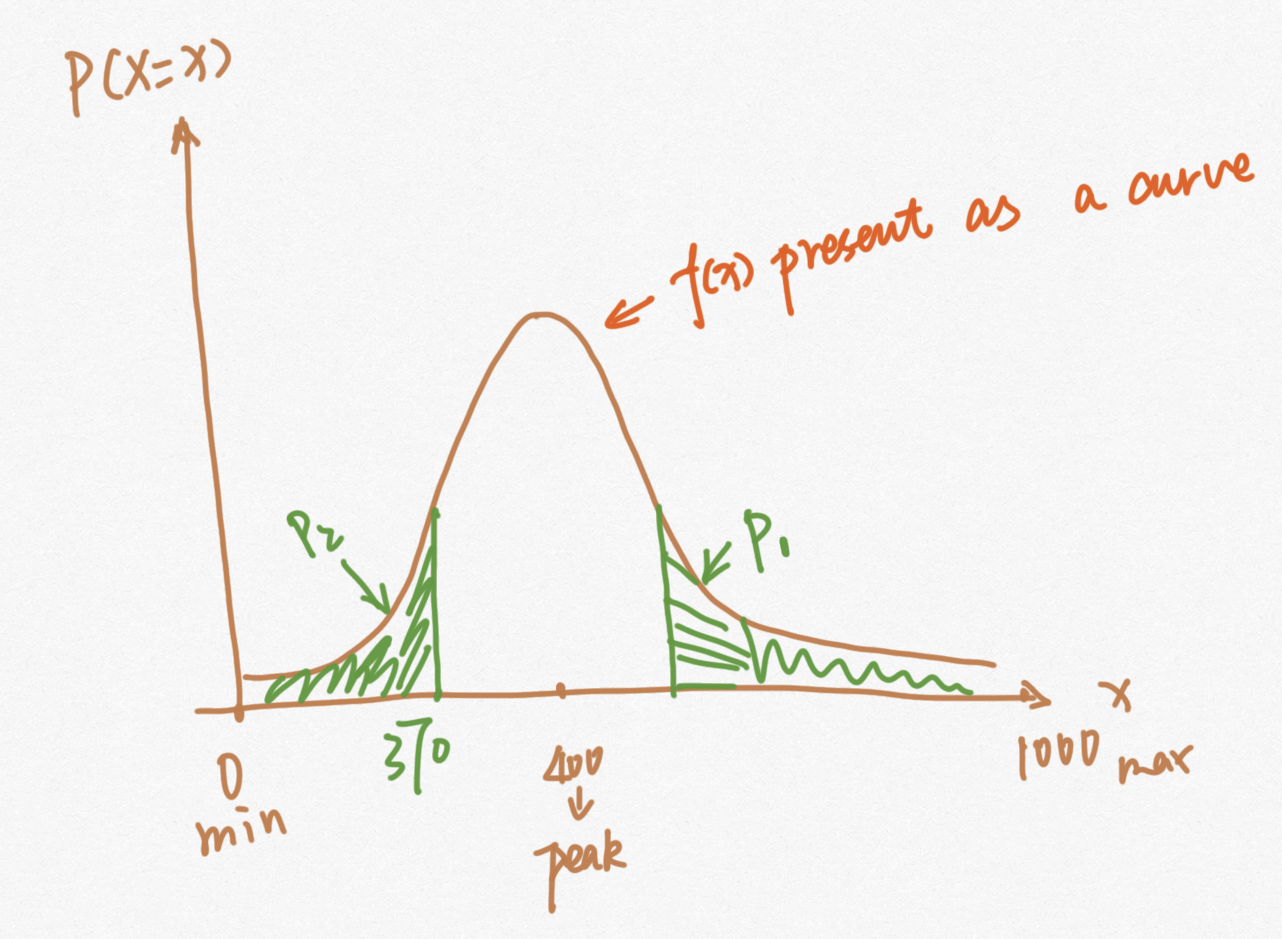
\includegraphics[width=0.8\linewidth]{1c}
				\label{fig:1c}
			\end{figure}
			\item For the $p$-value, \begin{align*}
				\mathbb{P}(X\leq 370) & = F_X(370)
			\end{align*}
			The $R$ code for the $p$-value is \qquad  \texttt{2 * pbinom(370,1000,0.4)}
			\item If the  true value of $p$ is 0.4, just around $5.6\%$ of the time the polling of $1000$ people will give an answer as extreme as $x = 370$. This $p$-value is slightly greater than $0.05$ and it's non-significant, therefore we have no evidence against the null hypothesis that $p = 0.4$ at $5\%$ level of significance. The observed polling is \textbf{compatible} with possibility that the true support for Ardent is $40\%$.
			\item If the opinion poll has National polling at $41\%$ and Labour polling at $37\%$, this does not mean that National is definitely ahead of Labour. As we have shown in previous questions, given the sample with $41\%$ and $37\%$ polling respectively, we do not have evidence to against the null hypothesis which both Parties have $40\%$ supporters from the sample population. \\
			We could not tell whether one party's supporter is more than the other from the testing we did above. 
		\end{enumerate}
		\item \begin{enumerate}[label = (\alph*)]
			\item Let X be the number of Peters-voter out of $1000$ respondents. \begin{align*}
				X & \sim \text{Binomial}(1000, P_p)\\
				H_0 &: P_p = 0.05 \\
				H_1 &: P_p \neq 0.05 & \text{(two-sided test)}
			\end{align*}
			\item Under $H_0$, we have $X \sim \text{Binomial}(1000,0.05)$. The probability function of $X$ peaks at about $1000 \times 0.05 = 50$
			\begin{figure}[H]
				\centering
				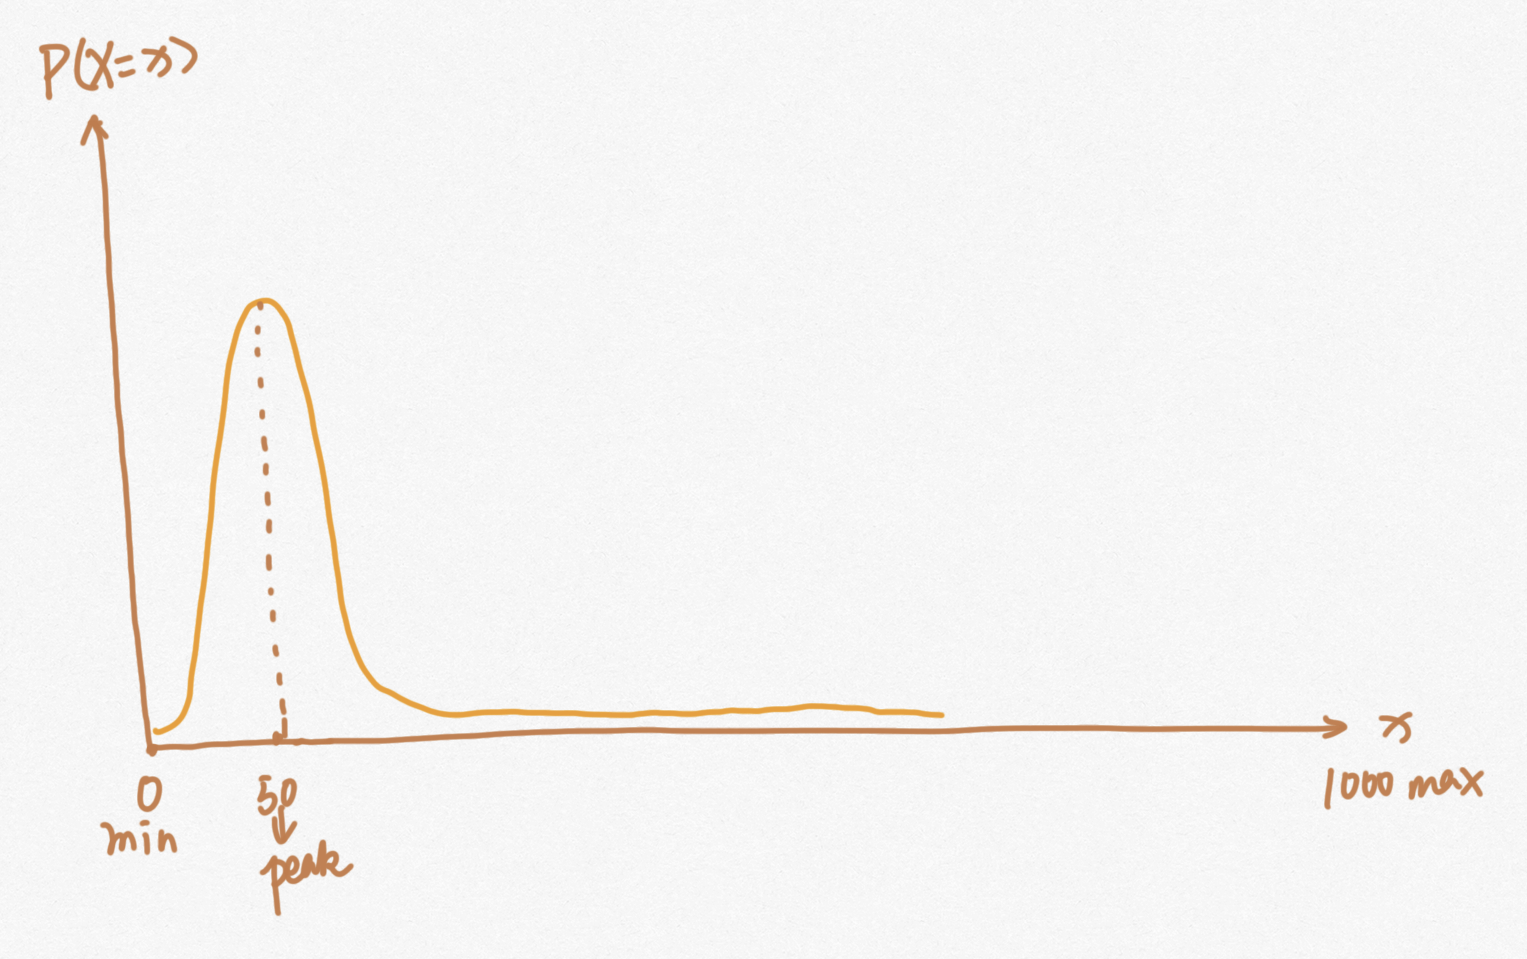
\includegraphics[width=0.8\linewidth]{2b}
				\label{fig:2b}
			\end{figure}
			\item \begin{figure}[h]
				\centering
				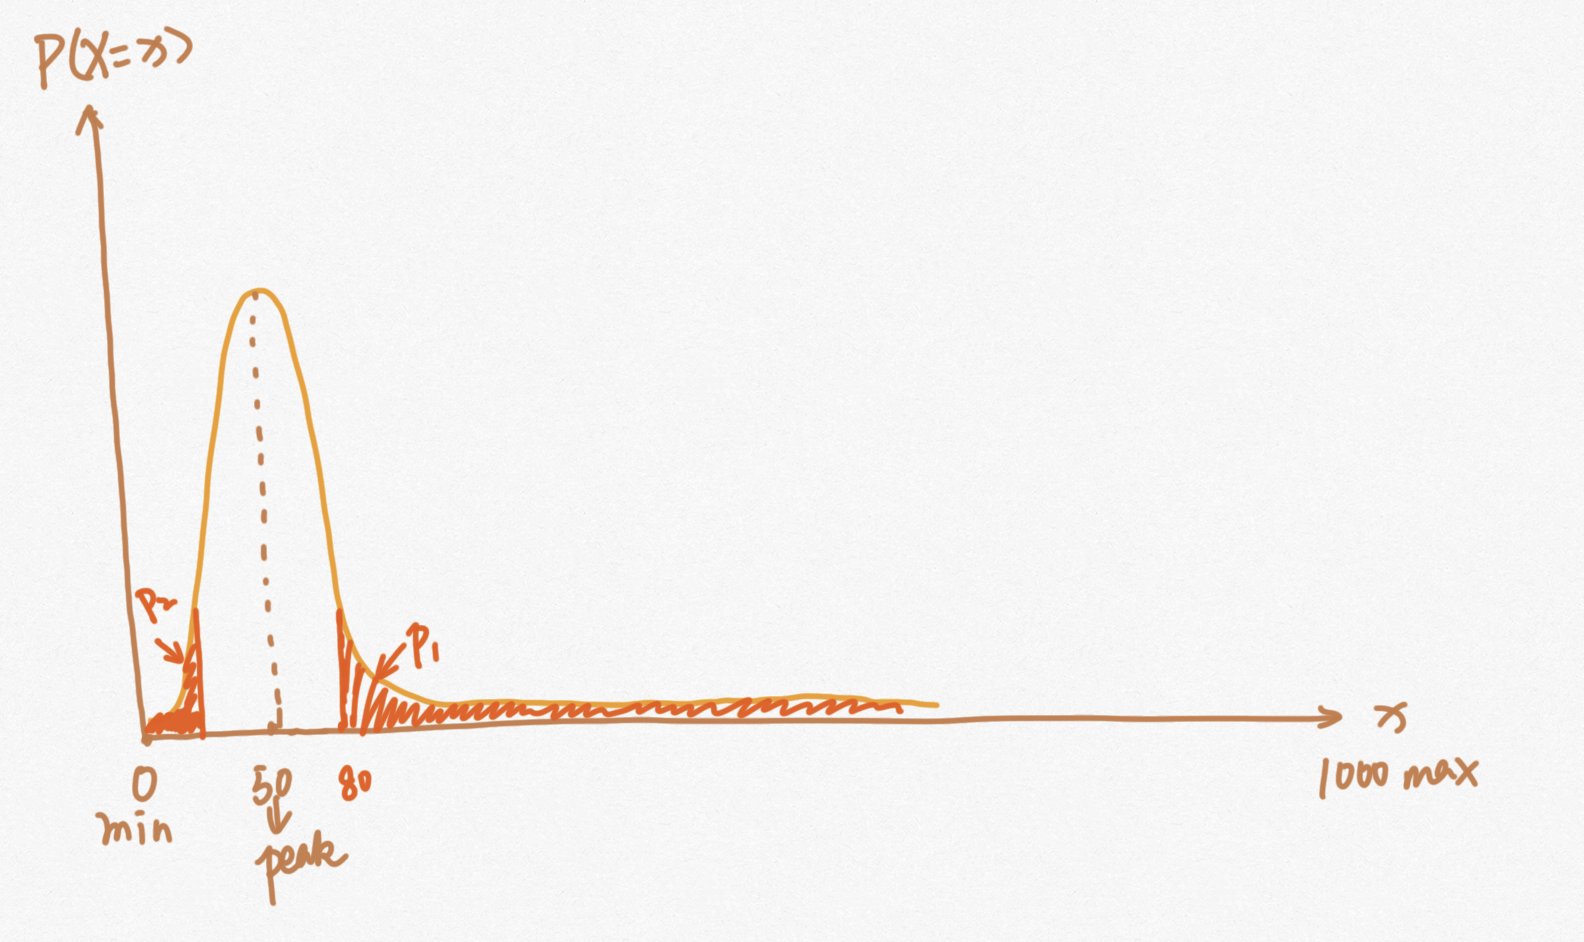
\includegraphics[width=0.8\linewidth]{2c}
				\label{fig:2c}
			\end{figure}
			\item For the p-value, \begin{align*}
				\mathbb{P}(X \geq 80)  & = 1 - \mathbb{P}(X < 80) \\
				& = 1 - \mathbb{P}(X \leq 79) \\
				& = 1 - F_X(79)
			\end{align*}
			The $R$ code for the $p$-value is \qquad \texttt{2 * (1 - pbinom(79,1000,0.05))}
			\item If the true value of $p$ is $0.05$, we have close to $0\%$ of the chance to see that out of $1000$ people will vote for Peters as extreme as $x = 80$. This $p$-value is very small and therefore we have strong evidence against the null hypothesis that $p = 0.05$. The observed polling is \textbf{not compatible} with the possibility that the true support for Peters is $5\%$.
			\item The conclusion is not the same. For 1(e), we are testing the true $p$ is a right shift of $3$ percentage points away from the observed polling, we have no evidence to against our $H_0$. While 2(e) we are testing the true $p$ is a left shift of $3$ percentage points away from the observed polling and we have strong evidence to against our $H_0$. \\
			I think it's our hypothesis is different. In 1(e) we are testing whether the true supporter is about $40\%$, but 2(e) we are testing against the worst-scenario.
		\end{enumerate}
	\end{enumerate}
\end{document}